The system allows different kinds of user to perform different actions. In particular:
\begin{itemize}
	\item Visitors can simply register or log in.
	\item Logged user can reserve and rent a car, plug a car into a safe area and finally communicate with the customers service in case of any problems during one of this operations
\end{itemize}
The user's action as the all the sequence is it possible to do with them is explain in the figure \ref{fig:UseCasesDiagram}

\subsection{Goals}
Here are described the software's high level goals:
\begin{enumerate}[label=\subscript{G}{\arabic*}]
	\item Allow visitor to sign up
	\item Allow user to log in
	\item Allow user to rent a car
	\item Allow user to book a car in a certain location
	\item Allow user to see the reservation?s confirmation and the time of expiration
\end{enumerate}

\subsection{UML}
\begin{figure}[H]
   \begin{center}
    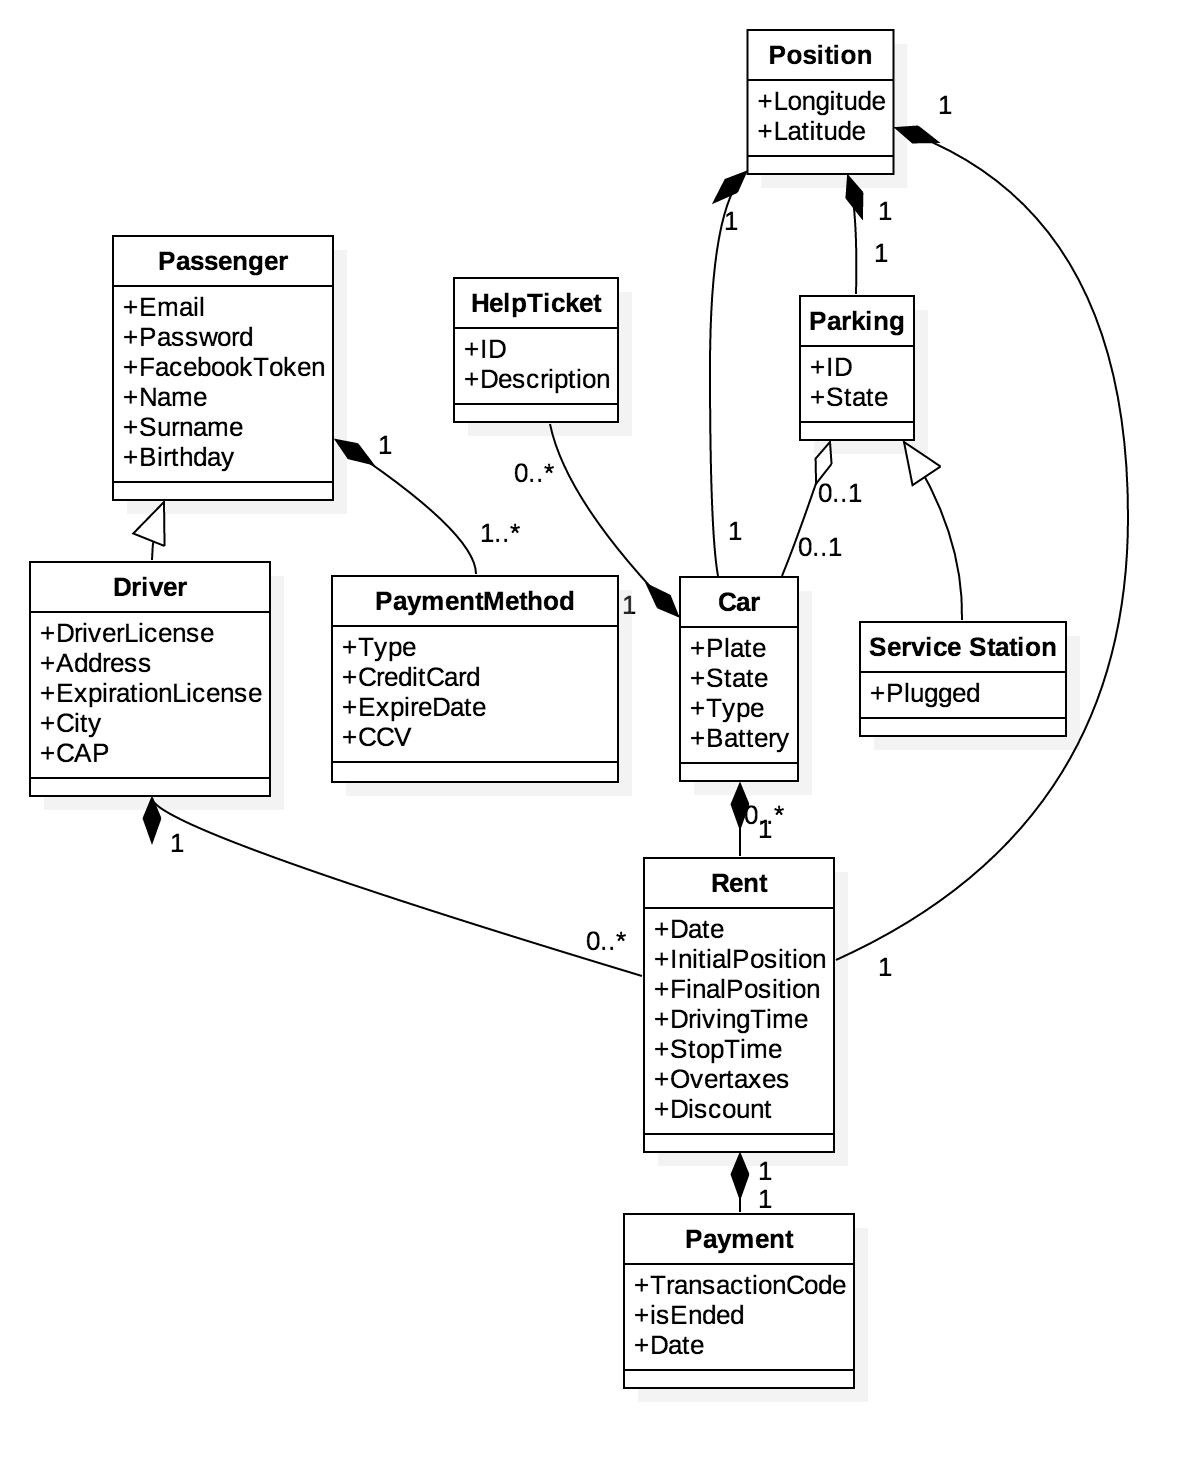
\includegraphics[width=\textwidth]{Resources/UML.png}
    \caption{Class Diagram}
   \end{center}
    \label{fig:ClassDiagram}
\end{figure}
\vfill
\vfill
